\section{Career Paths}
\label{sect:career-paths}
The goal of the career paths module is to generate data, such that a web user
interface could generate a nodal graph of the career paths taken to reach the
specified career goal.  The node transitions along with the transition
frequencies are returned to the user interface as objects.  Additionally,
the node ordering and information about each individual node is also returned in
an object.  This information can then be used to generate a nodal map
depicting various ways of achieving a career goal.  

An example is depicted in figure \ref{fig:nodal map}, which shows various
interconnected nodes that eventually arrive at the goal node.  The nodes are
arranged such that the user most likely travels from left to right, but the
occasional infrequently traveled transition may flow in the reverse direction. 
The frequency that the the path is traveled is depicted through line thickness
in this example.  Each node would then be able to display the individual node
information upon user request; either through clicking on the node or through
some other user action.  Note, that ProGENitor does not limit the method in
which the user interface is displayed; it simply passes back statistical
information about the nodes, the transitions between each node, and the
individual data about each node.  It is up to the web user interface developer
to determine how the end product is rendered.


\usetikzlibrary{shapes,arrows,chains}

\begin{figure}[H]
	\centering
  
% Start the picture
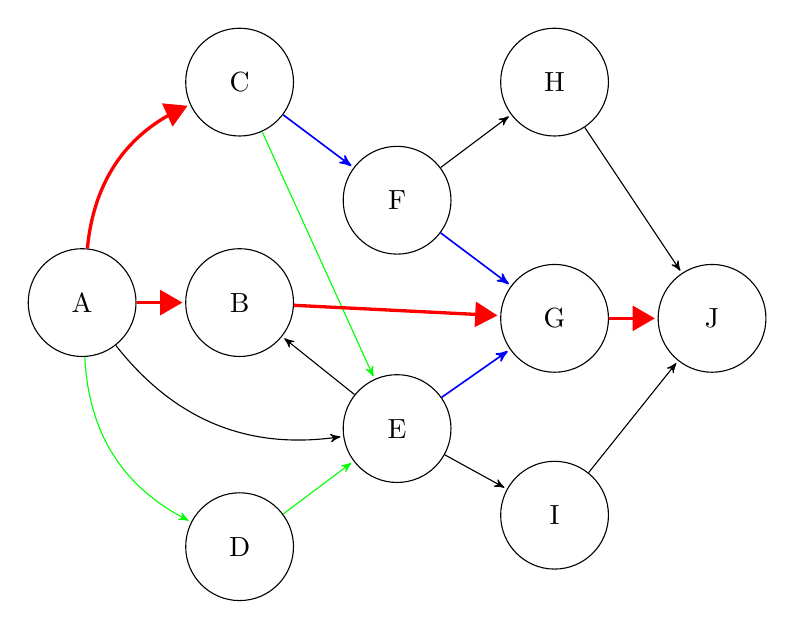
\begin{tikzpicture}[%
    >=triangle 60,              % Nice arrows; your taste may be different
    start chain=going below,    % General flow is top-to-bottom
    node distance=3mm and 20mm, % Global setup of box spacing
    every join/.style={norm},   % Default linetype for connecting boxes
    ]
% ------------------------------------------------- 
% A few box styles 
% <on chain> *and* <on grid> reduce the need for manual relative
% positioning of nodes
\tikzset{
  base/.style={draw, on chain, on grid, align=center, minimum height=2ex},
  node/.style={base, circle, text width=3em},
  % Connector line styles for different parts of the diagram
  norm/.style={->, draw},
  thin/.style={->,>=stealth',shorten >=1pt, black},
  nm/.style={->,>=stealth',shorten >=1pt, green},
  to/.style={->,>=stealth',shorten >=1pt,semithick,blue},
  thick/.style={->,shorten >=1pt,very thick, red},
  it/.style={font={\small\itshape}}
}
% -------------------------------------------------
% Start by placing the nodes
\node [node] (a) {A};
% Use join to connect a node to the previous one 
\node [node, right = of a] (b) {B};
\node [node, above = of b, yshift=25mm] (c) {C}; 
\node [node, below of = b, yshift=-25mm](d) {D};
\node [node, right=of d, yshift =15mm](e) {E};
\node [node, right=of c, yshift=-15mm](f) {F};
\node [node, right=of f, yshift=-15mm](g) {G};
\node [node, right=of f, yshift=15mm](h) {H};
\node [node, right=of f, yshift=-40mm](i) {I};
\node [node, right=of g](j) {J};

\draw[thick] (a) to (b);
\draw[thick] (a) to[bend left=30] (c);
\draw[nm] (a) to[bend right=30] (d);
\draw[nm] (d) to (e); 
\draw[thin] (a) to[bend right=30] (e);
\draw[nm] (c) to (e);
\draw[to] (c) to (f);
\draw[thin] (e) to (b);
\draw[to] (e) to (g);
\draw[to] (f) to (g);
\draw[thick] (b) to (g);
\draw[thin] (f) to (h);
\draw[thin] (e) to (i);
\draw[thick] (g) to (j);
\draw[thin] (h) to (j);
\draw[thin] (i) to (j);

% -------------------------------------------------
\end{tikzpicture}

	\caption{Career Path Graph}
	\label{fig:nodal map}
\end{figure}

\subsection{Graph Edges}
The graph edges portion of code finds all of the nodes that
users pass through and the order at which they pass through them.  It then
tallies the number of times all of the users pass along each transition
path to allow for the career path graph to depict not only the point to point
connections, but also how frequently that edge is traveled.  The high level
process to generate this graph interconnection data is depicted in figure
\ref{fig:node interconnect}.


\usetikzlibrary{shapes,arrows,chains}

\begin{figure}[H]
	\centering
% Start the picture
\resizebox {!} {110mm} {
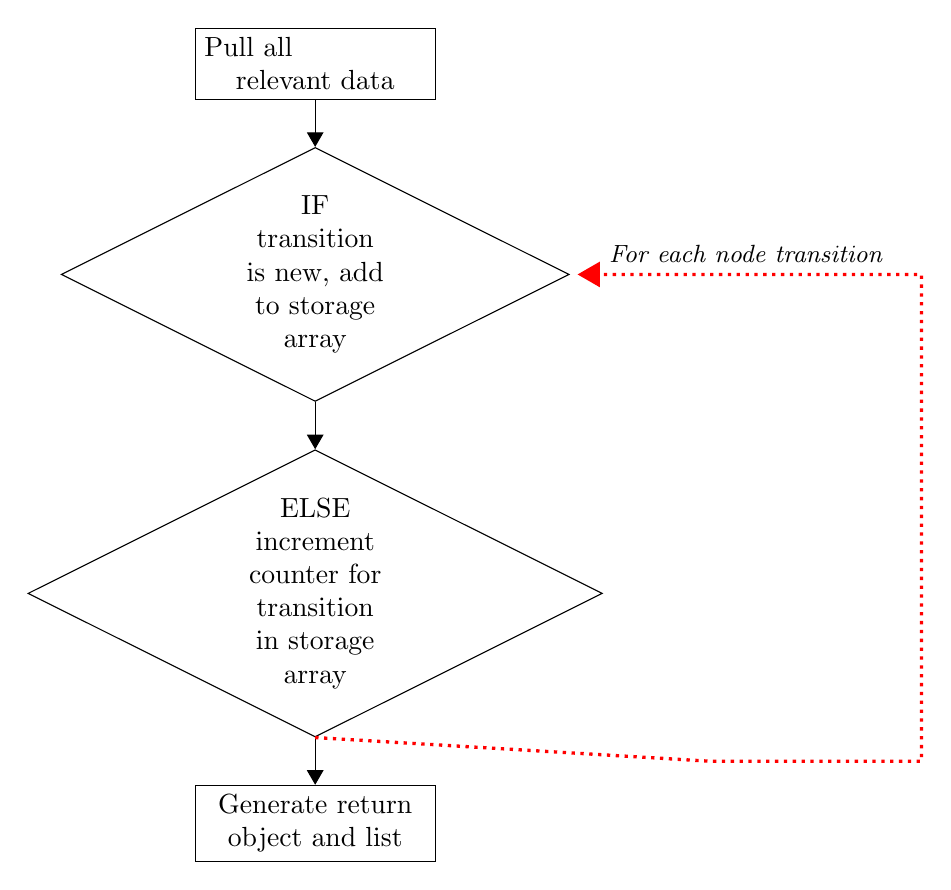
\begin{tikzpicture}[%
    >=triangle 60,              % Nice arrows; your taste may be different
    start chain=going below,    % General flow is top-to-bottom
    node distance=6mm and 60mm, % Global setup of box spacing
    every join/.style={norm},   % Default linetype for connecting boxes
    ]
% ------------------------------------------------- 
% A few box styles 
% <on chain> *and* <on grid> reduce the need for manual relative
% positioning of nodes
\tikzset{
  base/.style={draw, on chain, on grid, align=center, minimum height=4ex},
  proc/.style={base, rectangle, text width=8em},
  test/.style={base, diamond, aspect=2, text width=5em},
  % Connector line styles for different parts of the diagram
  norm/.style={->, draw},
  it/.style={font={\small\itshape}}
}
% -------------------------------------------------
% Start by placing the nodes
\node [proc] (p0) {Pull all\newline relevant data};
% Use join to connect a node to the previous one 
\node [test, join] (t1) {IF transition is new, add to storage array};
\node [test, join] (t2) {ELSE increment counter for transition in storage
array}; 
\node [proc, join](p1) {Generate return object and list};

\draw [->, dotted, thick, shorten >=1mm]
  (t2.south) -- ++(50mm,-3mm)  -- ++(27mm,0) 
  |- node [black, near end, yshift=0.75em, it]
    {For each node transition} (t1);

% -------------------------------------------------
\end{tikzpicture}
}
	\caption{High Level Graph Edge Generation}
	\label{fig:node interconnect}
\end{figure}

\noindent The process flow in defining and counting these edges is listed
in detail below:

\begin{description}
    \item[Graph Edge Generation:]
\end{description}
\begin{enumerate}
  \item For each ID passed to edge generation module:
  \begin{enumerate}
    \item Pull job data and add it to the nodes list.
    \item Pull education data and add it to the nodes list.
    \item Set Min equal to Max Integer and Max equal to MIN Integer.
    \item For each element of the nodes list:
    \begin{enumerate}
      \item If date of data for element of nodes is less than Min and more than
      Max, store the data and set Min equal to date of data.
      \item After all elements of nodes list considered, add stored data
      to user list and set Max equal to Min.
  	\end{enumerate}
  	\item For each element of user list:
  	\begin{enumerate}
  	  \item If A is NULL, set A equal to user element node name.
  	  \item Else set B equal to A and set A equal to user element node name.
  	  \item If edges list is empty, add B,A,1 to edges list.
  	  \item Else check if B,A exists in the edges list:
  	  \begin{enumerate}
  	    \item If it exists, increment the counter of the row.
  	    \item If it does not exist, add B,A,1 to the edges list.
  	  \end{enumerate}
  	\end{enumerate}
  \end{enumerate}
  \item Push edges list containing all graph transitions and transition
  counts to an object containing an array.
  \item Return both the list and the object.
\end{enumerate}

\subsection{Node Ordering}
The node ordering portion of code sorts the nodes such that the major
transitions flow in order from start to finish. It does this so that the flow
of transitions can be graphed in a manner that is not overly confusing.  Figure
\ref{fig:node ordering} shows the high level process that the code follows
to generate the node groupings.  These groupings can then be fed to the end user
interface to order the nodes in a fashion that shows the typical flow of careers
that reach the destination goal.

\usetikzlibrary{shapes,arrows,chains}

\begin{figure}[H]
	\centering
	\resizebox {!} {145mm} {
% Start the picture
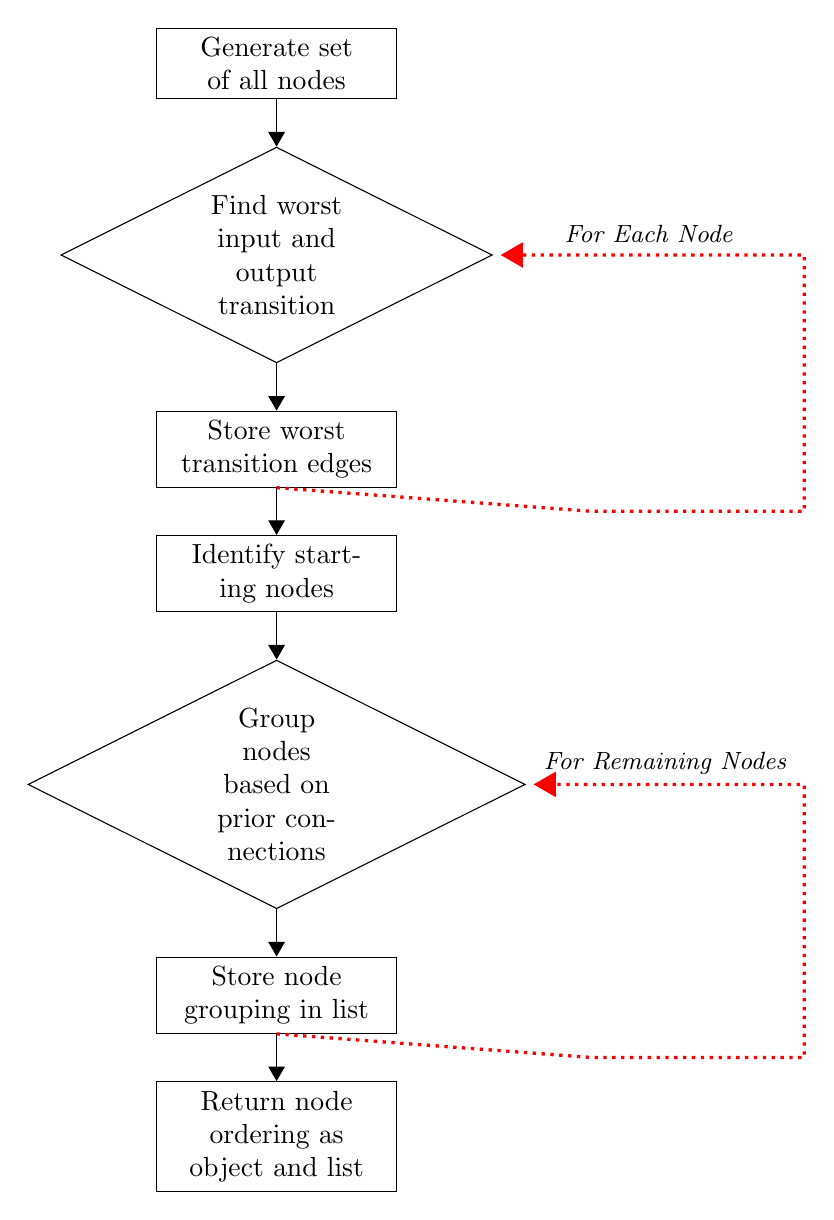
\begin{tikzpicture}[%
    >=triangle 60,              % Nice arrows; your taste may be different
    start chain=going below,    % General flow is top-to-bottom
    node distance=6mm and 60mm, % Global setup of box spacing
    every join/.style={norm},   % Default linetype for connecting boxes
    ]
% ------------------------------------------------- 
% A few box styles 
% <on chain> *and* <on grid> reduce the need for manual relative
% positioning of nodes
\tikzset{
  base/.style={draw, on chain, on grid, align=center, minimum height=4ex},
  proc/.style={base, rectangle, text width=8em},
  test/.style={base, diamond, aspect=2, text width=5em},
  % Connector line styles for different parts of the diagram
  norm/.style={->, draw},
  it/.style={font={\small\itshape}}
}
% -------------------------------------------------
% Start by placing the nodes
\node [proc] (p0) {Generate set of all nodes};
% Use join to connect a node to the previous one 
\node [test, join] (p1) {Find worst input and output transition};
\node [proc, join] (p2) {Store worst transition edges};
\node [proc, join] (p3) {Identify starting nodes}; 
\node [test, join] (p4) {Group nodes based on prior connections};
\node [proc, join] (p5) {Store node grouping in list};
\node [proc, join] (p6) {Return node ordering as object and list};

\draw [->, dotted, thick, shorten >=1mm]
  (p2.south) -- ++(40mm,-3mm)  -- ++(27mm,0) 
  |- node [black, near end, yshift=0.75em, it]
    {For Each Node} (p1);
\draw [->, dotted, thick, shorten >=1mm]
  (p5.south) -- ++(40mm,-3mm)  -- ++(27mm,0) 
  |- node [black, near end, yshift=0.75em, it]
    {For Remaining Nodes} (p4);

% -------------------------------------------------
\end{tikzpicture}
}
	\caption{High Level Node Order Generation}
	\label{fig:node ordering}
\end{figure}

\noindent The process flow in defining the node ordering for the nodes is listed
in detail below:

\begin{description}
    \item[Node Ordering Generation:]
\end{description}
 \begin{enumerate}
   \item Generate set of all nodes
   \item For each node in set:
   \begin{enumerate}
     \item Initialize transitional weight to 0.
     \item For each element of the graph edge list:
     \begin{enumerate}
       \item Check if node matches the input node.
       \item Check if the number of transitions to the node is greater than the
       transitional weight.
       \item If both checks are true; set the transitional weight to the current
       list line's number of transitions.
       \item Also, if both checks are true; store this list line.
     \end{enumerate}
     \item After the worst input transition is found for the node, store it in
     the heavy edges set.
     \item Repeat this entire step for the output nodes.
   \end{enumerate}
   \item For each heavy edge element, search the graph edge list
   for input nodes that are also destination nodes.
   \begin{enumerate}
     \item Any nodes not found are set as start nodes.
     \item Repeat this step for output nodes that are also starting nodes.  Any
     nodes not found are set as ending nodes.
   \end{enumerate}
   \item Add all the starting nodes to node 0 and add them to the node store
   set.
   \item Add all nodes that are not starting nodes to the remaining nodes
   set.
   \item Increment the group number to 1.
   \item Until the remaining nodes set is empty, loop through the following
   steps.
   \begin{enumerate}
     \item For each node in node store, store all destination nodes in a set
     that node in node store transitions to.
     \item For each destination node stored in the previous step, find all
     possible next destination nodes and check if they are contained within the
     set generated in the previous step.
     \begin{enumerate}
       \item If one is contained within the previously generated set, remove
       the node from the set.
     \end{enumerate}
     \item Add remaining nodes to next node grouping.  Also remove remaining
     nodes from remaining nodes set.
     \item Add the node group to the node return list.
     \item Increment the group number.
     \item Replace the nodes in the starting nodes set with the nodes that
     were just added to a group.
   \end{enumerate} 
   \item Generate an object containing an array of the node groupings from
   the node return list.
   \item Return both the object and the node return list.
 \end{enumerate}



\subsection{Node Details}
Presenting all of the potential information would overwhelm any user interface,
so instead many of the details are buried within each node and can be queried
by the end user, by selecting the node of interest.  As each node contains
additional details such as the place of employment or education, time spent at
the school or job, or any other node relevant pieces of information; the data
must be gathered upon user request, as to not slow down the overall graph
generation.  Once the request is made, the data about the individuals who
reached the goal node and the data about all of the users who passed through a
particular node are pulled.  This data is then broken down into a statistic for
both cases and compared against each other to determine if something occurred
more frequently for the users who reached the goal node versus those who had
not.  This way any significant differences could be raised to the end user's
attention as potentially important steps to reaching the final goal.  The high
level process to generating this data is depicted in figure \ref{fig:node
details}.

\usetikzlibrary{shapes,arrows,chains}

\begin{figure}[H]
	\centering
% Start the picture
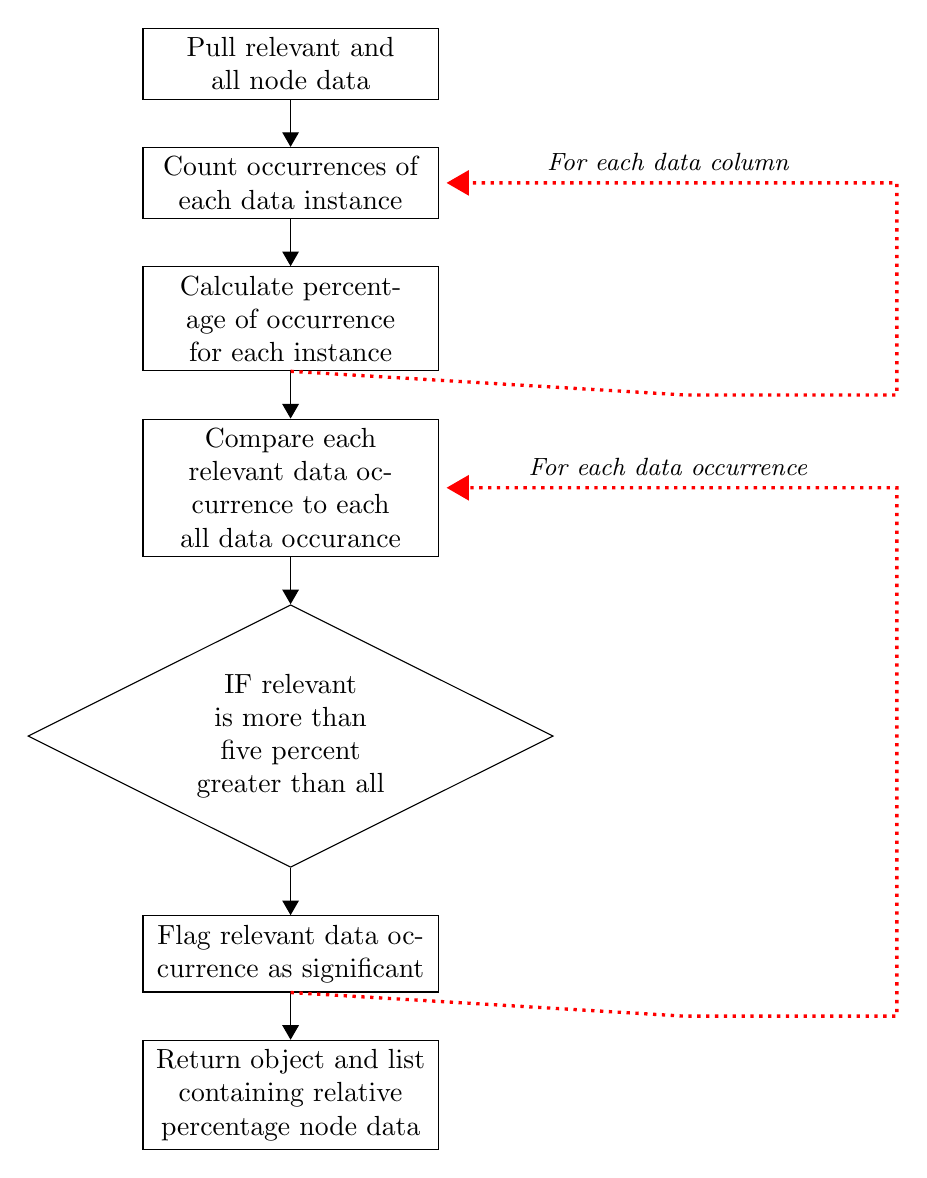
\begin{tikzpicture}[%
    >=triangle 60,              % Nice arrows; your taste may be different
    start chain=going below,    % General flow is top-to-bottom
    node distance=6mm and 60mm, % Global setup of box spacing
    every join/.style={norm},   % Default linetype for connecting boxes
    ]
% ------------------------------------------------- 
% A few box styles 
% <on chain> *and* <on grid> reduce the need for manual relative
% positioning of nodes
\tikzset{
  base/.style={draw, on chain, on grid, align=center, minimum height=4ex},
  proc/.style={base, rectangle, text width=10em},
  test/.style={base, diamond, aspect=2, text width=8em},
  % Connector line styles for different parts of the diagram
  norm/.style={->, draw},
  it/.style={font={\small\itshape}}
}
% -------------------------------------------------
% Start by placing the nodes
\node [proc] (p0) {Pull relevant and all node data};
% Use join to connect a node to the previous one 
\node [proc, join] (p1) {Count occurrences of each data instance};
\node [proc, join] (p2) {Calculate percentage of occurrence for each
instance};
 \node [proc, join] (p3) {Compare each relevant data occurrence to each all data
 occurance};
 \node [test, join] (t0) {IF relevant is more than five percent greater than
 all};
 \node [proc, join] (p4) {Flag relevant data occurrence as significant};
 \node [proc, join] (p5) {Return object and list containing relative percentage node data};

\draw [->, dotted, thick, shorten >=1mm]
  (p2.south) -- ++(50mm,-3mm)  -- ++(27mm,0) 
  |- node [black, near end, yshift=0.75em, it]
    {For each data column} (p1);
\draw [->, dotted, thick, shorten >=1mm]
  (p4.south) -- ++(50mm,-3mm)  -- ++(27mm,0) 
  |- node [black, near end, yshift=0.75em, it]
    {For each data occurrence} (p3);

% -------------------------------------------------
\end{tikzpicture}
	\caption{High Level Node Detail Generation}
	\label{fig:node details}
\end{figure}
\pagebreak

\noindent The process flow in defining the details and significant details for
each node is listed in detail below:

\begin{description}
    \item[Node Detail Generation:]
\end{description}
\begin{enumerate}
  \item Pull in profile list, tag each element as a profile, and then add
  the element to the complete list.
  \item Repeat this for the jobs list and the education list.
  \item Check each element of the complete list.
  \begin{enumerate}
    \item If the element contains the node that details are being pulled on, add
    the element to the relevant list.
  \end{enumerate}
  \item Pull the headers associated with the node that details are being pulled
  from.
  \item Pull all the data in the database for that node and store in the all
  node data list.
  \item For each element of the complete list:
  \begin{enumerate}
    \item Split the element into columns and step through each column.
    \begin{enumerate}
    	\item Check if the column element is a start or end year and instead
    	calculate the years spent at the node.
    	\begin{enumerate}
    	  \item If the end year is set to current, find the current year and then
    	  calculate the total years spent at the node.
    	\end{enumerate}
    	\item Add the column value to a set to obtain all possible values for
    	the column.
    	\item Step through the column counting each value instance to obtain a
    	count for each different value.
    	\item Calculate the percentage for each value in the column by diving the
    	count by the total number of elements.
    	\item Push these values into the relevant list.
    \end{enumerate} 
  \end{enumerate}
  \item Repeat for each element of the all node data list
  \item Compare the percentages for each element of the relevant list to
  the percentages from the all node data list.
  \begin{enumerate}
    \item Flag the column value for any instance where the relevant value's
    percentage exceeds the percentage for all the data by 5\%.
    \item Return this value as relevant so that it can be identified to the user
    as significant to the node.
  \end{enumerate}
  \item Return the relevant list and an object containing an array
  of the same data.
\end{enumerate}
\pagebreak

